% % -*- coding:utf-8 -*-
\documentclass[aspectratio=169,10pt]{beamer}
\nonstopmode

%\documentclass[handout,aspectratio=169,10pt]{beamer}
%\usepackage{pgfpages}
%\pgfpagesuselayout{2 on 1}[a4paper,border shrink=5mm]

\usepackage{appendixnumberbeamer}
\setbeamertemplate{footline}[frame number]
\usepackage{graphicx}
\usepackage{tikz}
\usepackage{url}
%\usepackage{mathrsfs} 
%\usepackage{unicode-math} 
%\setmathfont{XITS Math}
% color palette
\definecolor{tu01}{HTML}{84B818}
\definecolor{tu02}{HTML}{D18B12}
\definecolor{tu03}{HTML}{1BB5B5}
\definecolor{tu04}{HTML}{F85A3E}
\definecolor{tu05}{HTML}{4B6CFC}
\definecolor{tu06}{HTML}{E3B505}
\definecolor{tu07}{HTML}{AF331D}
\definecolor{tu08}{HTML}{000000}
\definecolor{tu09}{HTML}{AAAAAA}
\definecolor{tu10}{HTML}{444444}
\definecolor{tu11}{HTML}{84B818}

% mixed and light colors
\colorlet{tu01light}{tu01!33}
\colorlet{tu02light}{tu02!33}
\colorlet{tu03light}{tu03!33}
\colorlet{tu04light}{tu04!33}
\colorlet{tu05light}{tu05!33}
\colorlet{tu06light}{tu06!33}
\colorlet{tu07light}{tu07!33}
\colorlet{tu08light}{tu08!33}
\colorlet{tu09light}{tu09!33}
\colorlet{tu10light}{tu10!33}
\colorlet{tu11light}{tu11!33}

\colorlet{tu01midlight}{tu01!50}
\colorlet{tu02midlight}{tu02!50}
\colorlet{tu03midlight}{tu03!50}
\colorlet{tu04midlight}{tu04!50}
\colorlet{tu05midlight}{tu05!50}
\colorlet{tu06midlight}{tu06!50}
\colorlet{tu07midlight}{tu07!50}
\colorlet{tu08midlight}{tu08!50}
\colorlet{tu09midlight}{tu09!50}
\colorlet{tu10midlight}{tu10!50}
\colorlet{tu11midlight}{tu11!50}

\colorlet{tu01dark}{tu01!80!black}
\colorlet{tu02dark}{tu02!80!black}
\colorlet{tu03dark}{tu03!80!black}
\colorlet{tu04dark}{tu04!80!black}
\colorlet{tu05dark}{tu05!80!black}
\colorlet{tu06dark}{tu06!80!black}
\colorlet{tu07dark}{tu07!80!black}
\colorlet{tu08dark}{tu08!80!black}
\colorlet{tu09dark}{tu09!80!black}
\colorlet{tu10dark}{tu10!80!black}
\colorlet{tu11dark}{tu11!80!black}

\colorlet{lightgray}{gray!25}
\colorlet{midlightgray}{gray!50}
\colorlet{anthracite}{black!85}

% aliases
\colorlet{tudo}{tu01}
\colorlet{tuorange}{tu02}
\colorlet{tudolight}{tu01light}

% math
\definecolor{data}{RGB}{230, 128, 3}
\definecolor{functions}{RGB}{47, 50, 204}
\definecolor{params}{RGB}{64, 179, 53}
\definecolor{paramsigma}{RGB}{179, 179, 7}

\newcommand{\smally}{{\color{data}y}}
\newcommand{\bigy}{{\color{data}Y}}
\newcommand{\smallx}{{\color{data}x}}
\newcommand{\boldx}{{\color{data}\textbf{x}}}
\newcommand{\boldy}{{\color{data}\textbf{y}}}
\newcommand{\bigx}{{\color{data}\textbf{X}}}
\newcommand{\trainset}{{\color{data}\mathcal{D}}}
\newcommand{\predy}{{\color{data}\hat{y}}}
\newcommand{\basisF}{{\color{data}\Phi}}
\newcommand{\classset}{{\color{data}\mathcal{C}}}
\newcommand{\aclass}{{\color{data}c}}

\newcommand{\paramw}{{\color{params}w}}
\newcommand{\paramW}{{\color{params}\textbf{w}}}
\newcommand{\estimw}{{\color{params}\hat{w}}}
\newcommand{\estimW}{{\color{params}\hat{\textbf{w}}}}
\newcommand{\estsigma}{{\color{paramsigma}\sigma}}
\newcommand{\estSigma}{{\color{paramsigma}\hat{\sigma}}}

\newcommand{\func}{{\color{functions}f}}
\newcommand{\funcg}{{\color{functions}g}}
\newcommand{\basisf}{{\color{functions}\phi}}


\newcommand{\argmax}[1]{\underset{#1}{\operatorname{arg}\,\operatorname{max}}\;}
\newcommand{\argmin}[1]{\underset{#1}{\operatorname{arg}\,\operatorname{min}}\;}


% \usepackage{beamerthememetropolis}
\usetheme[progressbar=frametitle]{metropolis}
\newcommand{\themename}{\textbf{\textsc{metropolis}}\xspace}


\usepackage{xcolor}


\title{Machine Learning and Intelligent Systems}
\subtitle{Introduction}
\author{Maria A. Zuluaga}

\institute{EURECOM - Data Science Department}
\titlegraphic{\hfill
\includegraphics[height=15mm]{images/logo_eurecom.jpg}}

\date{October 4, 2022}

\begin{document}

\maketitle
%\begin{frame}{Table of contents}
%	\tableofcontents
%\end{frame}
%TODO Table of contents
%\item Tutorial for Beamer \url{https://www.overleaf.com/learn/latex/Beamer_Presentations:_A_Tutorial_for_Beginners_(Part_1)%E2%80%94Getting_Started}
%	\item Quelle Template: \url{https://github.com/matze/mtheme}
%	\item Quelle Bild: \url{https://unsplash.com/photos/52gEprMkp7M}





\section{Introduction to Machine Learning}

\begin{frame}[t]{Traditional Computer Science vs. Machine Learning}
	\centering
	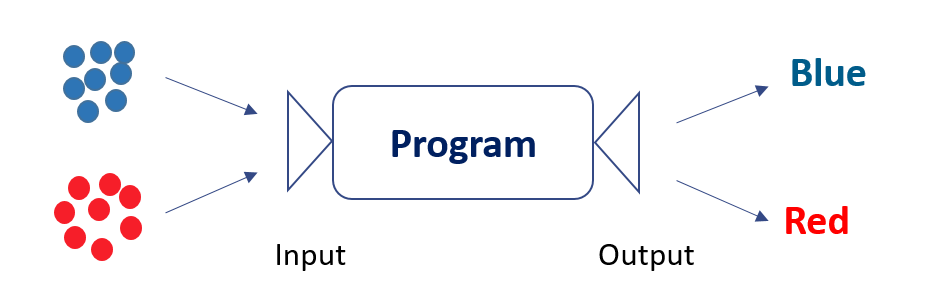
\includegraphics[width=0.7\linewidth, clip]{images/pc_program}\\
	Traditional Way \\
	\pause
	\vspace{0.2cm}
	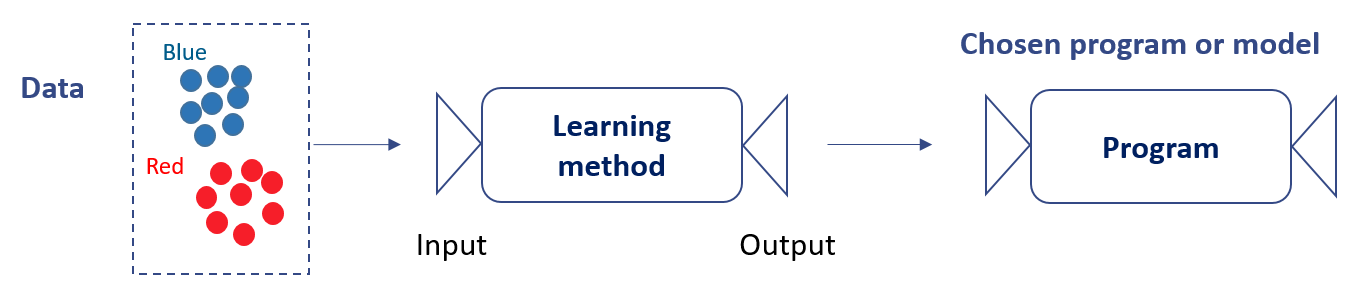
\includegraphics[width=0.85\linewidth, clip]{images/ml}\\
	Machine Learning
\end{frame}

\begin{frame}{Machine Learning: Definition}
	\begin{columns}
		\column{0.7\textwidth}
		\begin{itemize}
			\item Term introduced in 1959 by Arthur L. Samuel [1]
			\pause 
			\vspace{0.3cm}
			\item Formal definition (Tom M. Mitchell [2]):
			
			A computer program is said to learn from experience $E$ with respect to some class of tasks $T$ and performance measure $P$ if its performance at tasks in $T$, as measured by $P$, improves with experience $E$.
			
		\pause \vspace{0.3cm}
			\item In simple words: Algorithms that improve on a task with experience	
		\end{itemize}
	\vspace{0.8cm}
{\footnotesize [1] A. Samuel. Some studies in machine learning using the game of Checkers. IBM Journal of Research and Development (1959)} %}\\
%	\vspace{-0.2cm}
%	{\tiny

	{\footnotesize	[2] T.M. Mitchel. Machine Learning (1997)}
		\column{0.3\textwidth}
		\centering
		\onslide
			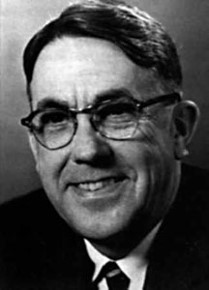
\includegraphics[width=0.4\linewidth, clip]{images/arthur_samuel}\\
			\vspace{-0.2cm} 
			{\tiny Arthur Samuel (1901-1990)}\\
			\vspace{0.3cm}
			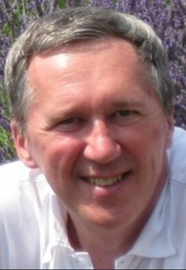
\includegraphics[width=0.4\linewidth, clip]{images/tom_mitchell}\\
				{\tiny Tom M. Mitchell}\\
				\vspace{-0.2cm} 
				{\tiny Computer Scientist and}\\
				\vspace{-0.2cm} 
				{\tiny Professor @CMU}
	\end{columns}
 
\end{frame}



\begin{frame}{Machine Learning: Learning from Data}
	\alert{An example:} Spam filtering
	\begin{itemize}
		\item Task ($T$):
		\item Experience ($E$):
		\item Performance measure ($P$):
	\end{itemize}

\pause
Learning from experience (i.e. data) to be able to:
\begin{itemize}
	\item Make predictions
	\item Find similarities
	\item Find patterns 
	\item Discover knowledge
\end{itemize}

{\tiny Example adapted from: T. Mitchell \url{http://www.cs.cmu.edu/afs/cs.cmu.edu/project/theo-20/www/mlbook/ch1.pdf}}
\end{frame}

\begin{frame}{Some history}
	\centering
	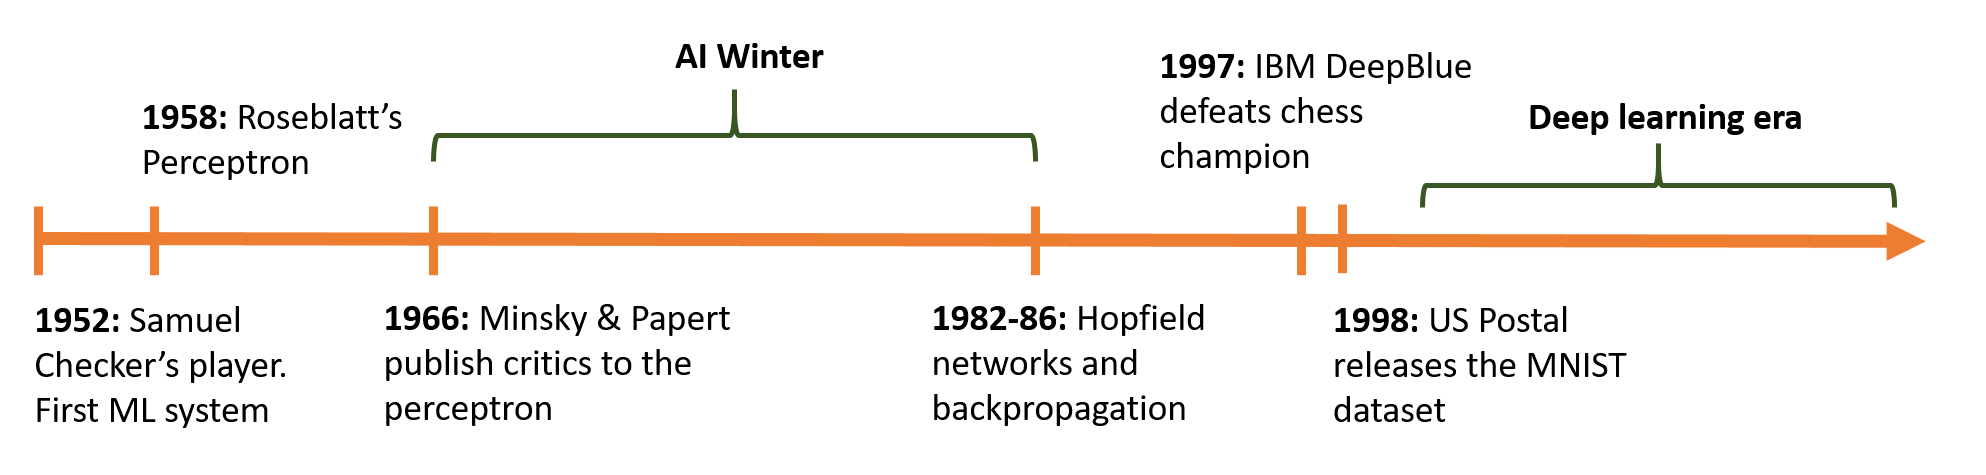
\includegraphics[width=\linewidth, clip]{images/ai_history}
\end{frame}

\begin{frame}{AI vs. Machine Learning}
	\begin{columns}[t]
		\column{0.33\textwidth}
		\begin{center}\textbf{AI (before AI winter)}\end{center}
		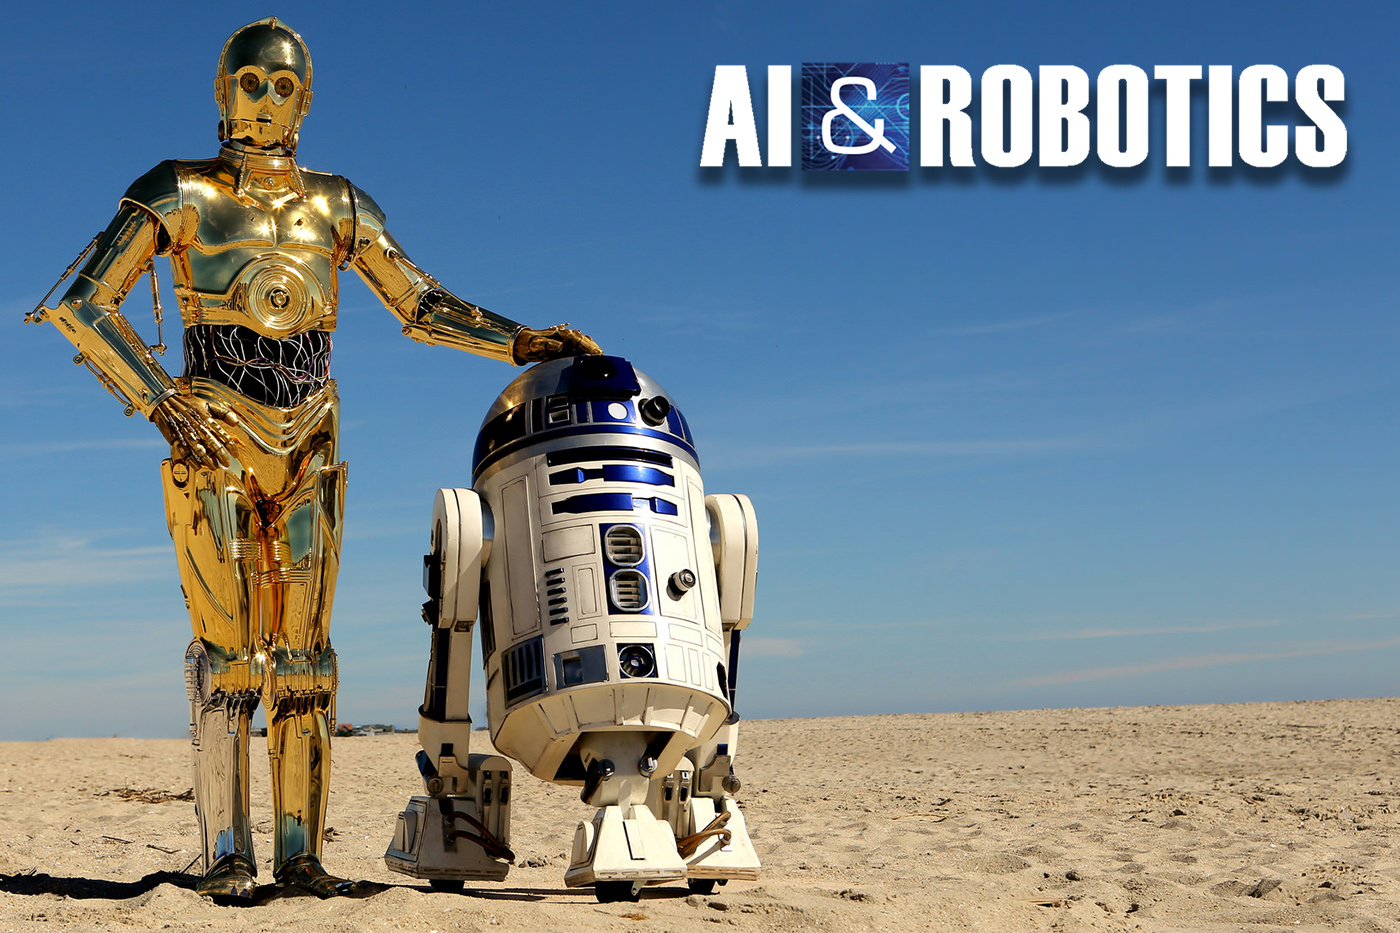
\includegraphics[width=\textwidth, clip]{images/ai_before}\\
		\begin{itemize}
			\item Top-down approach
			\item Based on logic
		\end{itemize}
	
		\column{0.33\textwidth}
		\begin{center}\textbf{Machine Learning}\end{center}
			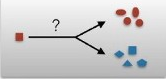
\includegraphics[width=0.9\textwidth, clip]{images/ml_simple}\\
		\begin{itemize}
			\item Firstly, a way to get funding
			\item Bottom-up approach: Starts from smaller goals
			\item Based on statistics and optimization
		\end{itemize}
		\column{0.33\textwidth}
	\begin{center}\textbf{AI in the DL era}\end{center}
	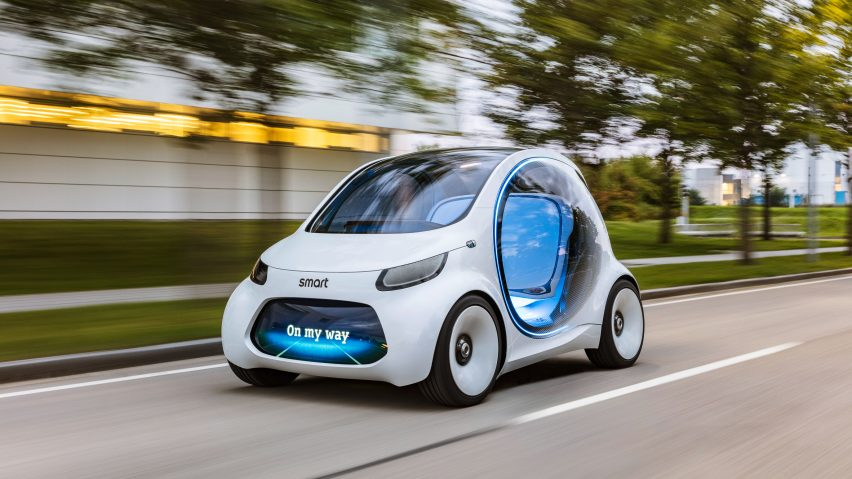
\includegraphics[width=0.9\textwidth, clip]{images/vehicle}\\
	\begin{itemize}
		%
		\item Term's rebirth: useful for funding 
		\item Result of last decades success
	\end{itemize}
	\end{columns}
\vspace{0.3cm}
{\tiny Adapted from K. Weinberg course @CMU}
\end{frame}
\begin{frame}{Key Issues in Machine Learning}
	\begin{itemize}
		\item What data (E) to use?
		\item How to represent it?
		\item Which algorithm should be used to learn?
		\item How to pick the best model?
		\item Can we be confident in the results?
		\item How to model a problem as a Machine Learning problem?
\end{itemize}
	
\end{frame}
\section{The Course}
\begin{frame}{What you will learn}
	\begin{itemize}
		\item Fundamental concepts underlying the mechanism of learning from data
		\item Several common algorithms to learn from data
		\item How to well-define a learning problem
		\item 	How to properly solve problems using these techniques
	\end{itemize}
\end{frame}

\begin{frame}{Types of Learning}
	\centering
	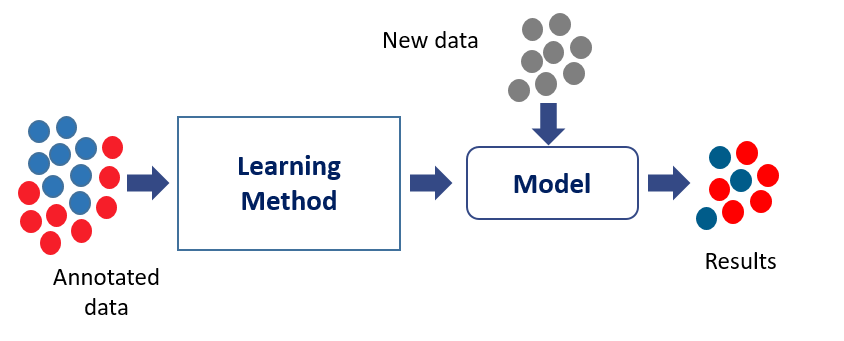
\includegraphics[width=0.6\linewidth, clip]{images/supervised}\\
Supervised Learning (80\%)\\
\pause
\vspace{0.2cm}
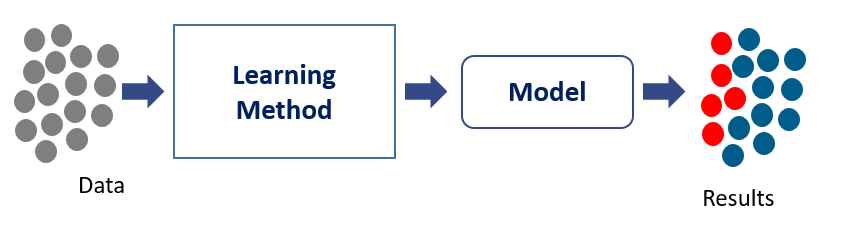
\includegraphics[width=0.6\linewidth, clip]{images/unsupervised}\\
Unsupervised Learning (20\%)
\end{frame}

\begin{frame}{Types of Learning: Reinforcement Learning}
	\begin{itemize}
		\item Learning what to do –how to map situations to actions to maximize a numerical reward.
		\item The learner is not told which actions to take, but must discover which yield the most reward.
		\item \alert{Examples:} Alpha GO, Robotics, Autonomous vehicles, resource management in computer clusters
	\end{itemize}
	\centering
	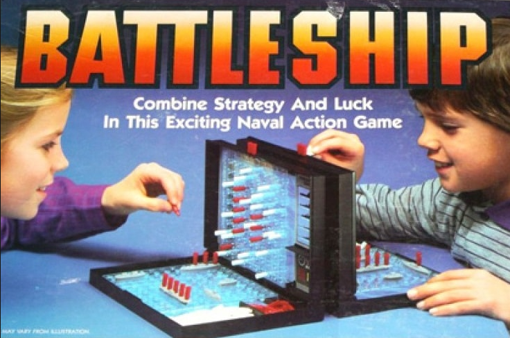
\includegraphics[width=0.4\linewidth, clip]{images/reinforcement}\\
	Not covered in this course
	\end{frame}
\begin{frame}{The Project}
	One of the main goals of this course is to prepare you to apply machine learning algorithms to real-world tasks, or to leave you well-qualified to start machine learning research. 
	
	The final project is intended to start you in these directions. You are expected to:
	\begin{itemize}
		\item Identify a problem that can be solved through the use of machine learning
		\item Choose an appropriate ML method 
		\item Propose and implement a solution
	\end{itemize}
	
\end{frame}

\begin{frame}{The Project}
	It is divided in four stages:
	\begin{enumerate}
		\item Project Proposal
		\item Project Progress report
		\item Final Deliverable 
		\item Final Presentation
	\end{enumerate}
\pause
\begin{alertblock}{First Assignment:}
	Visit \url{https://malis-course.github.io/project} and read the detailed description \\
\end{alertblock}
\begin{alertblock}{First Deliverable:}
	Project Proposal - Oct 17 (Moodle)
\end{alertblock}
\end{frame}

\section{Logistics}
\begin{frame}{Expected Previous Knowledge}
	Basic knowledge of:
	\begin{itemize}
		\item Probability
		\item Linear algebra
		\item Calculus
	\end{itemize}
	
	\vspace{1cm}
	For the labs, basic knowledge of:
	\begin{itemize}
		\item Programming
		\item Python - Labs run in Python
	\end{itemize}	
\end{frame}

\begin{frame}{Bibliography}
	\begin{columns}
		\column{0.7\textwidth}
		No official textbook followed.\\
		\vspace{1cm}
		Two suggested readings:
		\begin{itemize}
			\item \href{https://web.stanford.edu/~hastie/Papers/ESLII.pdf}{The Elements of Statistical Learning} – Hastie, Tibshirani, Friedman
			\item \href{https://www.microsoft.com/en-us/research/uploads/prod/2006/01/Bishop-Pattern-Recognition-and-Machine-Learning-2006.pdf}{Pattern Recognition and Machine Learning} – Bishop
		\end{itemize}
		\column{0.3\textwidth}
		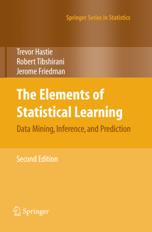
\includegraphics[width=0.55\linewidth, clip]{images/esl} \\
		\vspace{0.2cm}
		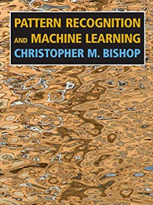
\includegraphics[width=0.55\linewidth, clip]{images/prml}
	\end{columns}
\end{frame}

\begin{frame}{Other resources (with links)}
	
	{\footnotesize \textbf{Machine Learning:}}
	\begin{itemize}
		{\footnotesize
			\item \href{http://web4.cs.ucl.ac.uk/staff/D.Barber/textbook/091117.pdf}{Bayesian reasoning and Machine Learning} – Barber
			\item \href{http://www.cs.huji.ac.il/~shais/UnderstandingMachineLearning/copy.html}{Understanding Machine Learning: From Theory to Algorithms} – Shalev-Shwartz \& Ben-David }
		    \item \href{http://noiselab.ucsd.edu/ECE228/Murphy_Machine_Learning.pdf}{\footnotesize Machine Learning a probabilistic perspective - Murphy}
	\end{itemize}

	{\footnotesize 	\textbf{Linear algebra:}}

\begin{itemize}
	{\footnotesize
		\item \href{http://cs229.stanford.edu/section/cs229-linalg.pdf}{Review notes from Stanford’s ML course} – Kolter \& Do
		\item \href{http://vmls-book.stanford.edu/vmls.pdf}{Introduction to Linear Applied Linear Algebra} – Boyd \& Vandenberghe}
\end{itemize}
	
	{\footnotesize \textbf{Probability:} 
			\href{http://cs229.stanford.edu/section/cs229-prob.pdf}{Review notes from Stanford’s ML course} – Maleki \& Do }
		

	{\footnotesize 	\textbf{Calculus:} 
			 \href{http://users.umiacs.umd.edu/~hal/courses/2013S_ML/math4ml.pdf}{Review notes from University of Maryland – Daumé III}}

	{\footnotesize \textbf{Python:} 
	\href{https://perso.limsi.fr/pointal/_media/python:cours:mementopython3-english.pdf}{Python cheat sheet} – Pointal }
	
\end{frame}

\begin{frame}{Modus Operandi}
	\textbf{10 lectures }
	\begin{itemize}
		\item Slides will be made available the Friday before the lecture in Moodle
		\item Slides with annotations will be available the next Friday following the lecture
		\item Some lectures will have accompanying code with exercises for you to complete (optional)
	\end{itemize}
	
	\textbf{4 labs:}
	\begin{itemize}
		\item Groups of 2 
	\end{itemize}
\end{frame}

\begin{frame}{Assessment}
	\begin{itemize}
		\item Labs : 10\%
		\item Project : 30\%
		\item Final exam : 60\%
	\end{itemize}
	
	\begin{block}{Important}
		To pass the course, every item grade needs to be greater or equal than 8.5
	\end{block}
\end{frame}

\begin{frame}[fragile]{Communication \& Contact}
	In order
	\begin{enumerate}
		\item Moodle: Forum and chat
		\item Mail: \verb|maria.zuluaga@eurecom.fr|
		\item Office hours: Thursdays 13.00 - 14.00 (Office 427)
	\end{enumerate}
	\begin{block}{Important}
		The main communication channel is the weekly lecture. If you fail to attend, it is your responsibility to find out about any announcement that has been made during the lecture.
	\end{block}
\end{frame}

\begin{frame}{Recommendation Letter Policy}
	Many students request a recommendation letter at the end of the term. I am fine with providing you a letter as long as the following two conditions are met:
	\begin{enumerate}
		\item Your final grade \textbf{at least} 15
		\item I know who you are
	\end{enumerate}

	Things I do not do:
	\begin{enumerate}
		\item Generic letters
		\item Provide you the letter
	\end{enumerate}
\end{frame}


	
\begin{frame}[t,standout]
	\Large
	Any questions?
\end{frame}

%\begin{frame}{Further Reading and Useful Material}
%	
%	\begin{table}
%		\begin{tabular}{|l | l | }
%			\hline
%			\multicolumn{1}{|c|}{\textbf{Source}} & \multicolumn{1}{c|}{\textbf{Notes}} \\
%			\hline
%			Samuel Checker's Player &	\href{https://link.springer.com/referenceworkentry/10.1007\%2F978-0-387-30164-8_740}{Encyclopedia of ML (link)} \\
%			Pattern Recognition and Machine Learning & Sec 1.5.5, Ch. 3 \\
%			\href{https://www.math.uwaterloo.ca/~hwolkowi/matrixcookbook.pdf}{The Matrix Cook Book} & \\
%			\href{http://vmls-book.stanford.edu/vmls.pdf}{Introduction to Linear Applied Linear Algebra}  & Part III – Least Squares\\
%			\hline
%		\end{tabular}
%	\end{table}
%	
%	
%\end{frame}

%\begin{frame}{Outlook}
%	\Large
%	The font size should be as large as possible
%	\begin{itemize}
%		\item \textit{Never smaller than the age of the oldest audience member}
%		\item Don't vary sizes to much, never within a slide
%		\item Stick to one font
%		\item Don't overuse formatting like bold, italics, alert, etc.
%	\end{itemize}
%	But you knew all that already...
%\end{frame}

\end{document}
